% !TeX root = ../main.tex

\chapter{Computación científica de alto rendimiento}
\begin{chapquote}{Alan Turing}
	``La idea detrás de los computadores digitales puede explicarse diciendo que estas máquinas están destinadas a llevar a cabo cualquier operación que pueda ser realizada por un equipo humano``
\end{chapquote}
En los anteriores capítulos se han dado definiciones y técnicas para generalizar los conceptos clásicos del cálculos en un contexto difuso, no obstante el objetivo final de este trabajo es encontrar y desarrollar métodos numéricos para resolver problemas en ecuaciones diferenciales difusas.

En este capítulo, \textbf{se tratan los problemas desde el punto de vista informático y se abordan distintas técnicas numéricas} que se van a aplicar en los capítulos posteriores para atacar estos problemas de la forma más eficiente posible. 

Este capítulo está basado en las notas que podemos ver en \cite{paralelo}.

\section{Conceptos básicos}
Dentro de la computación científica, podemos distinguir \textbf{una serie de conceptos esenciales}, que tienen que ver en cierta medida con las partes que forman un ordenador. Todo el mundo que tiene un ordenador, seguro que conoce ciertas partes de su ordenador, \textbf{memoria RAM, el procesador, tarjeta gráfica, tarjeta de red...} pero, ¿Qué impacto tiene cada uno de estos elementos en el desarrollo de la computación científica?

\subsection{Memoria RAM}
Los programas que se ejecutan en un ordenador se alojan en la memoria RAM, y una vez alojados en la memoria RAM, el procesador se encarga de procesar las instrucciones y ejecuta el código del programa procesando lo que se conoce como \textit{stack}. En resumen, \textbf{la memoria RAM es donde se almacenan las instrucciones que va a ejecutar el procesador, y todos los datos que generamos en nuestro sistema operativo.}
\\ 
La memoria RAM nos impone un límite de la cantidad de datos que puede estar en ejecución en un momento dado, y si se quiere obtener el máximo rendimiento posible, se tiene que \textbf{evitar escribir más memoria RAM de la disponible}, si no, el sistema operativo empezará a usar el disco duro para alojar información. Esta tecnología se le conoce como \textbf{\textit{swap}}, y es \textbf{mucho más lenta que la memoria RAM.}
\\ 
Dentro de un ordenador, se puede \textbf{dividir la memoria RAM en dos grupos}; \textbf{la memoria RAM disponible para el procesador}, y  \textbf{la memoria RAM disponible para la tarjeta gráfica}. Esto es bastante importante, pues cuando se trabaja con la \textbf{tarjeta gráfica, no se puede acceder a punteros alojados en la memoria RAM del procesador}, por tanto, \textbf{antes de acceder a esta información se debe copiar a la memoria RAM de la tarjeta gráfica.} La operación de copiar datos entre la memoria de la tarjeta gráfica al procesador es bastante lenta, y es conocido que en este punto existe \textbf{un cuello de botella.}
\\ 
Tener mucha memoria RAM en nuestra máquina también podría reducir el consumo energético, pues se reduciría el acceso al disco duro.

\subsection{Procesador (CPU)}
El procesador es la parte del ordenador que se encarga de interpretar las instrucciones que hemos generado con nuestro programa, y es también \textbf{fundamental a la hora de conseguir un rendimiento óptimo de un programa}. \\
Algunos de los aspectos a tener en cuenta para obtener un \textbf{mejor rendimiento serían los hilos del procesador, y los GHz}. Los \textbf{hilos del procesador permiten ejecutar tareas de manera simultanea}. Por ejemplo, si el procesador tiene $10$ hilos, y se quiere sumar un vector de $10$ elementos, se puede hacer que las 10 sumas que hacen falta para sumar el vector se hagan simultáneamente. En el caso de que se quieran hacer operaciones que dependan unas de otras podemos considerar un grafo árbol donde vamos procesando los nodos independientes de forma paralela y esperamos en los nodos dependientes hasta que todas las operaciones hayan sido realizadas.
\subsection{Tarjeta gráfica (GPU)}
Habitualmente, se piensa sólo en el mundo \textit{gaming} cuando se habla de tarjetas gráficas, y pensamos que su única utilidad es para jugar a videojuegos en alta resolución. Sin embargo, son más útiles de lo que puede parecer. \\ \\
En este caso, las gráficas podemos tratarlas de forma parecida a las CPU, sin embargo, la gran ventaja que ofrecen las GPU es que \textbf{están construidas para procesar muchos datos simultáneamente}, debido a que tienen \textbf{muchos más hilos disponibles que la CPU}. Pero por otro lado, \textbf{cada hilo es más lento.}

\subsection{Tarjeta de Red (Internet/Intranet/Cluster)}
Usar internet o intranet para trabajar con computación de alto rendimiento es una buena práctica. Esto es que cuando \textbf{conectamos varios ordenadores, llamados nodo, y los coordinamos para realizar una tarea. A este concepto se les llaman \textit{cluster de ordenadores}}. \\ \\
Es importante saber que la información a través de la tarjeta de red viaja \textbf{más lento que por las otras vías}, y hay otros factores a tener en cuenta, como la distancia física entre los ordenadores. Sin embargo, si queremos trabajar con \textbf{muchísimos hilos es la mejor opción que existe, esto es, conectar muchos ordenadores para realizar simultáneamente las operaciones que se le manden.}\\ \\
Tratemos de dar un símil con la vida real para esclarecer el funcionamiento. Pongamos que somos una empresa que vendemos productos por internet, donde hay miles de usuarios que hacen pedidos de forma simultaneas y queremos vender nuestros productos a toda España. Para ello necesitaríamos trabajar con servicios de mensajería. Cada servicio de mensajería podemos interpretarlo como un nodo de nuestro clúster, donde cada servicio de mensajería funciona de forma independiente pero tienen un objetivo común, que es cumplir la tarea que nosotros como empresa le hemos marcado.
\section{Técnicas de alto rendimiento}

Una vez introducidos los conceptos básicos acerca de los distintos elementos de la computación científica, vamos a hablar de las distintas técnicas que podemos abordar para \textbf{obtener un rendimiento lo más óptimo posible.}

\subsection{Programación de bajo nivel}
El \textbf{lenguaje de programación que utilicemos va a decantar la balanza en temas de rendimiento}. Si queremos exprimir al máximo nuestros ordenadores no nos quedará más remedio que decantarnos por lenguajes de más bajo nivel como C++ o C. Al no ser lenguajes interpretados, como pasa por ejemplo con Python, es decir, nuestro código se ejecuta directamente en nuestra máquina.

En las siguientes pruebas, vamos a revisar cómo se comportan Python y C, con el mismo código, en términos de tiempo de ejecución y de uso de RAM: (Ver código en el apéndice)

\begin{itemize}
\item \textbf{C es más eficiente a la hora de administrar la memoria RAM}, al probar 10000000000 iteraciones, \textbf{Python no puede reservar más memoria RAM, sin embargo, C es capaz de reservar la memoria necesaria sin ningún tipo de problema.}
  
\item Por otro lado, los tiempos de ejecución son más sorprendentes aún. \textbf{Con tan solo 10 iteraciones, C es 5 veces más rápido que Python, con $1000000$ iteraciones, C es 77 veces más rápido que Python y, finalmente, con $1000000000$ iteraciones, C es 100 veces más rápido que Python.} Aquí se ve la notable diferencia entre uno y otro. Si queremos trabajar en computación científica, trabajar con C debe ser nuestra primera elección. (Ver figura \ref{fig:cvspython})
\end{itemize}

\begin{figure}[h]
  \frame{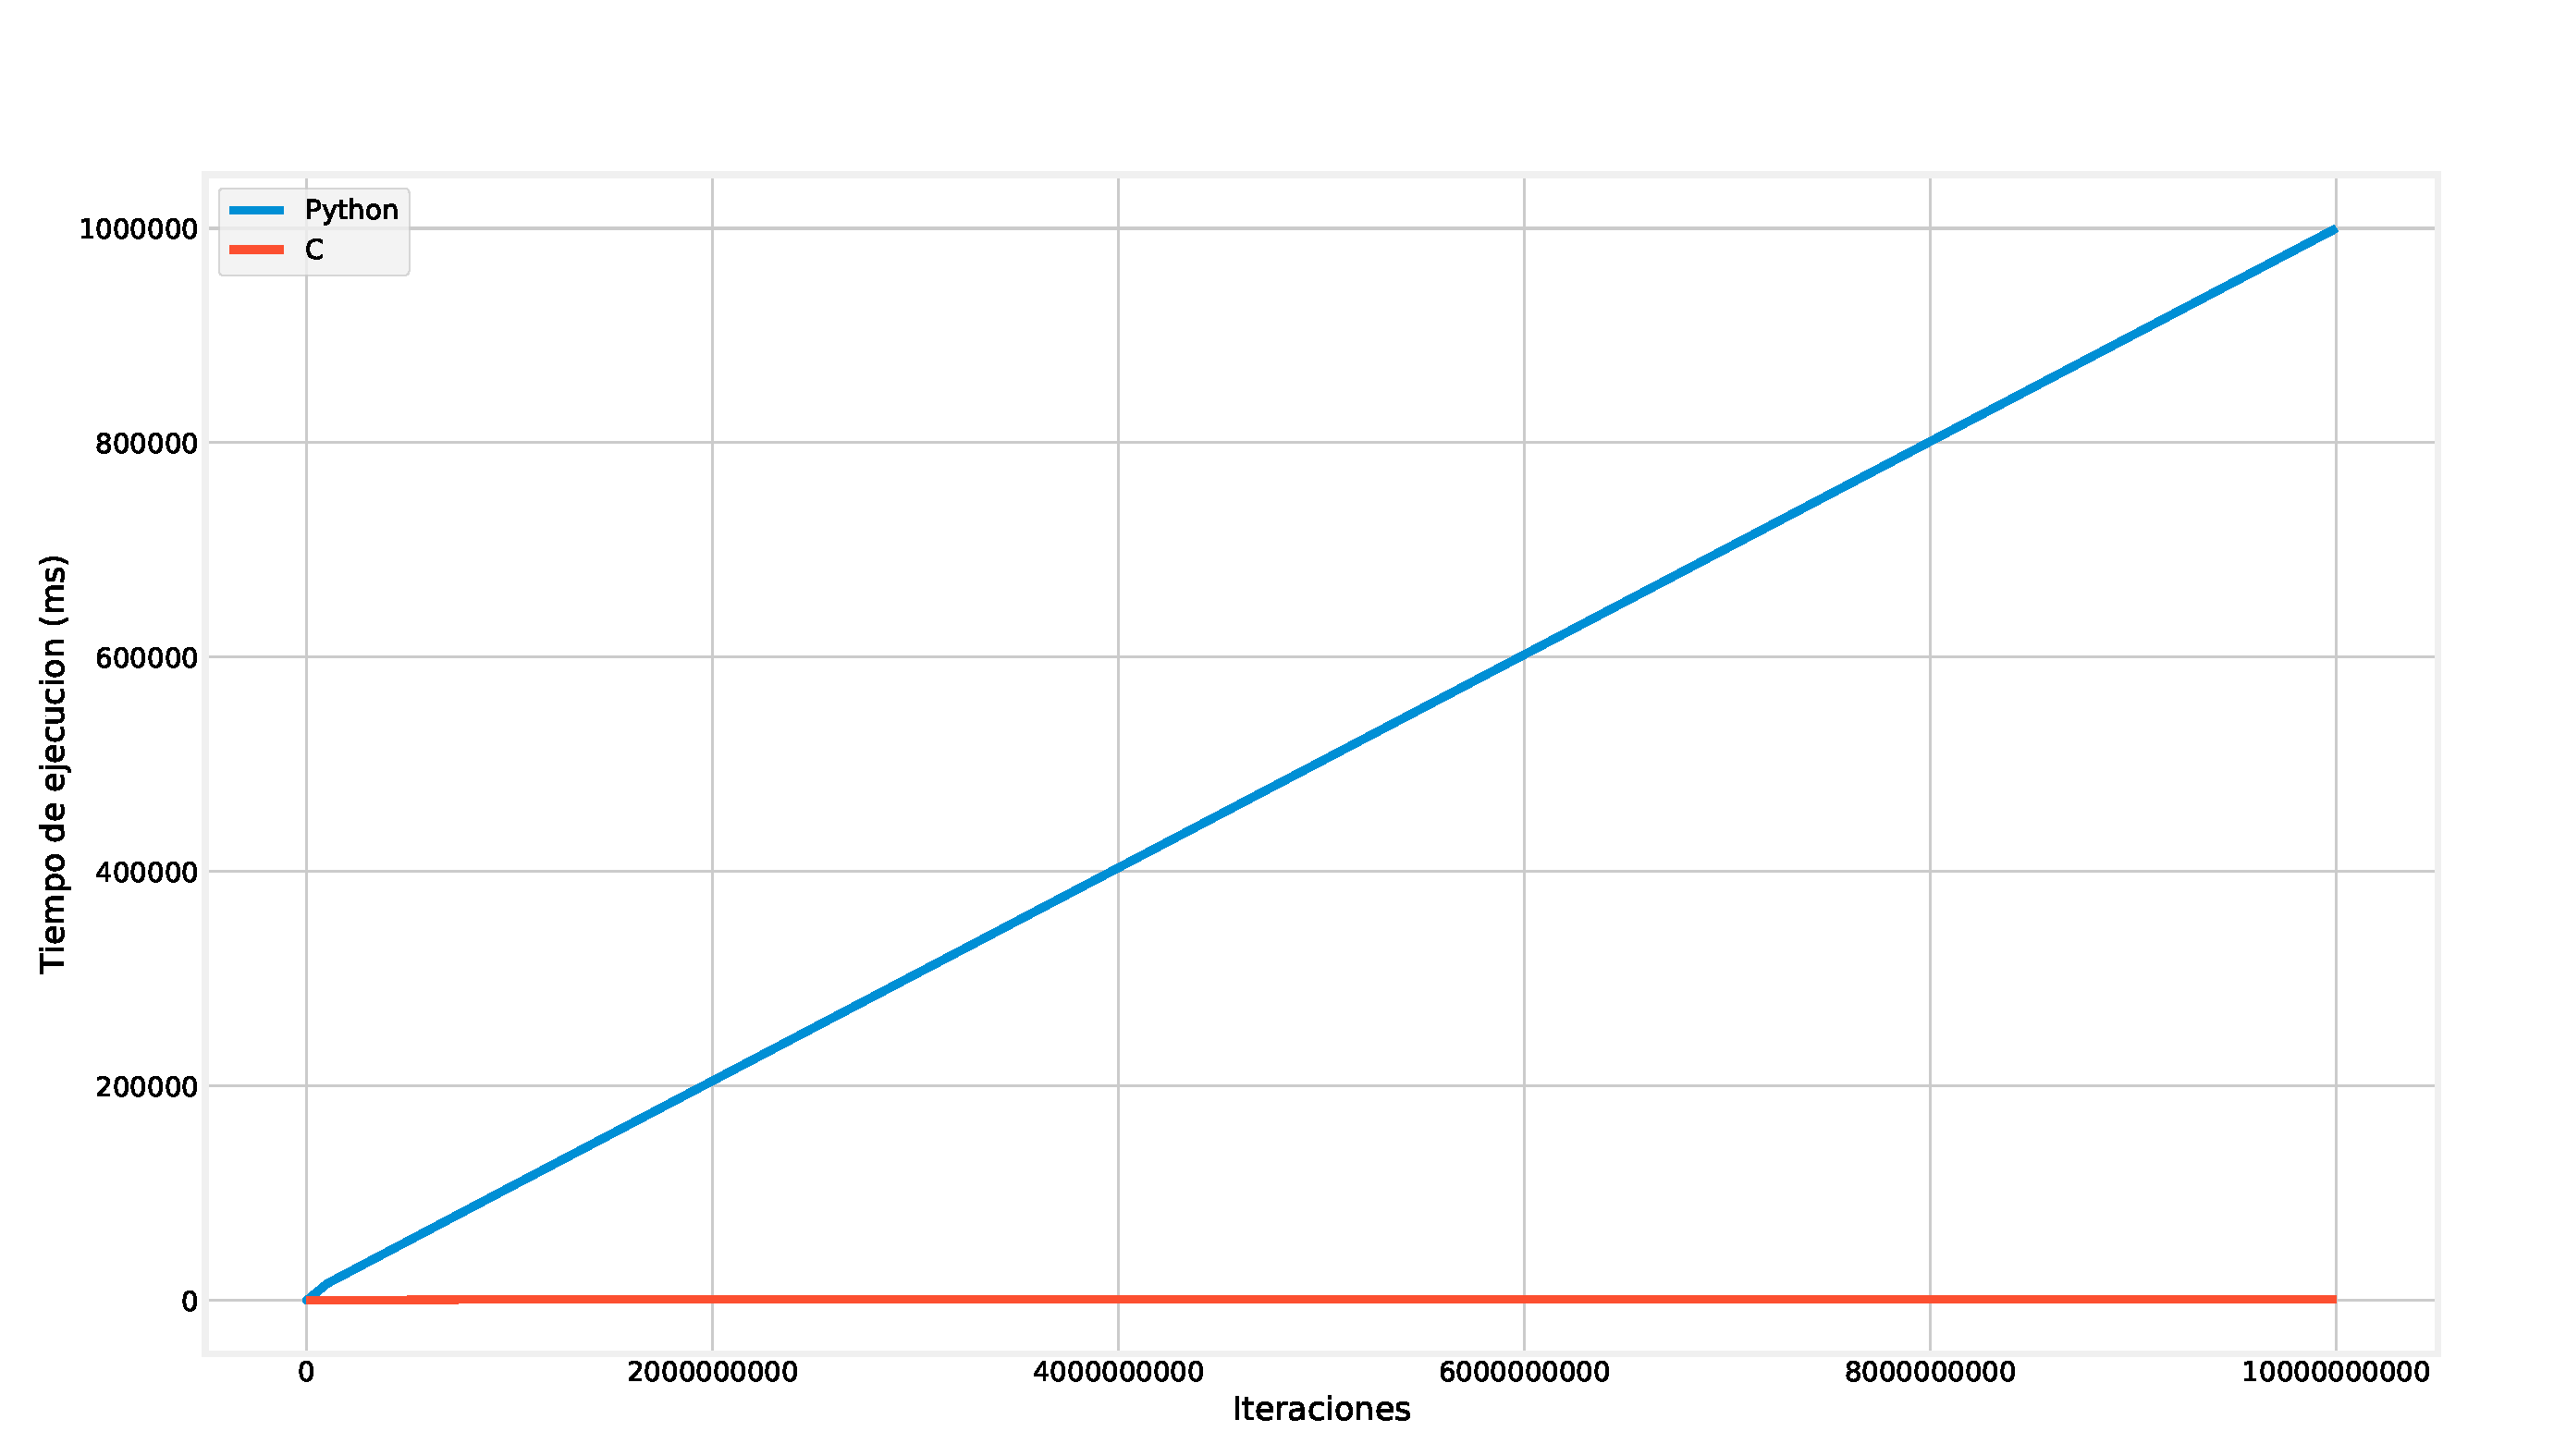
\includegraphics[width=\textwidth]{grafica_c_vs_python}}
  \centering
  \caption{Gráfica comparativa C vs Python \ref{prueba:simple_python}, \ref{prueba:simple_c}}
  \label{fig:cvspython}
\end{figure}

\subsection{Precisión mixta}
Otra técnica menos conocida, pero no por ello menos importante, es el uso de precisión mixta. Recordemos en primer lugar, que cuando trabajamos con números en un ordenador debemos de tener en cuenta la precisión con la que estamos trabajando. Existen algunas alternativas para trabajar con números en precisión \textit{<<infinita>>}, sin embargo, no son de nuestro interés pues no rinden tan bien como queremos, así que nos centraremos en dos tipos de precisiones:

\begin{itemize}
\item \textbf{Precisión simple: } Los números se representan utilizando 4 bytes, por tanto podemos representar $256^4$ combinaciones.
  
\item \textbf{Precisión doble: } Los números se representan utilizando 8 bytes, por tanto, podemos representar $256^8$ combinaciones.
\end{itemize}

Generalmente, los procesadores están optimizados para trabajar mejor con doble precisión. Las GPU suelen estar mejor optimizadas para trabajar con simple precisión, así que en estos casos, es útil tener en cuenta lo que llamamos precisión mixta si queremos tener un resultado en doble precisión. El procedimiento para trabajar con precisión mixta con un método iterativo es el siguiente:

\begin{itemize}
\item Planteamos en primer lugar nuestro problema de forma normal, y lo resolvemos realizando iteraciones en simple precisión.
\item Una vez que tenemos el resultado en simple precisión, inicializamos nuestro problema con el valor obtenido, a continuación realizamos iteraciones usando doble precisión.
\end{itemize}

A continuación, mostramos un ejemplo ilustrativo aplicando el método de Newton usando precisión mixta
\begin{ejemplo}[Método de Newton precisión mixta, comparativa y desarrollo]
  Supongamos que queremos encontrar las raices de la siguiente función:
  \[
  f(x) = (x-1)^8
  \]
  \[
  f'(x) = 8 (x-1)^7
  \]
  Nuestro objetivo es intentar conseguir una precisión que sea el cero de la máquina, en el sentido de que la diferencia entre dos iteraciones sea cero. En primer lugar resolveremos el problema en simple precisión, aplicando el método de Newton habitual:
  \begin{itemize}
  \item \textbf{Tiempo de ejecución: } 0m0,001s
  \item \textbf{Iteraciones en simple precisión: } 99
  \item \textbf{Iteraciones en doble precisión: } 0
  \item \textbf{Resultado: } 0.999998152256011962890625000000
  \end{itemize}

  Lo resolvemos ahora para doble precisión:
  \begin{itemize}
  \item \textbf{Tiempo de ejecución: } 0m0,001s
  \item \textbf{Iteraciones en simple precisión: } 0
  \item \textbf{Iteraciones en doble precisión: } 265
  \item \textbf{Resultado: } 0.999999999999999555910790149937
  \end{itemize}

  Si ahora resolvemos el problema aplicando los principios de la precisión mixta:
  \begin{itemize}
  \item \textbf{Tiempo de ejecución: } 0m0,001s
  \item \textbf{Iteraciones en simple precisión: } 99
  \item \textbf{Iteraciones en doble precisión: } 166
  \item \textbf{Resultado: } 0.999999999999999555910790149937
  \end{itemize}

  Podemos observar, que al resolver nuestro problema con precisión mixta hemos reducido en 100 las operaciones que tenemos que realizar en doble precisión, obteniendo una mejora de rendimiento. El código se puede encontrar en \ref{prueba:simple_c2}, \ref{prueba:doble_c2} y \ref{prueba:mixta_c2}
\end{ejemplo}

\subsection{Paralelización de algoritmos}
Una de las técnicas más conocidas para acelerar las operaciones que realizamos con un ordenador, es paralelizar los procesos.  Decimos que \textbf{un algoritmo de $n$ pasos se puede paralelizar} si cada iteración es independiente y el valor devuelto de esa iteración no depende del resto de iteraciones. \\
Para conseguir la paralelización, podemos hacerlo mediante diferentes tećnicas:

\begin{itemize}
\item \textbf{CPU:} Utilizando los hilos disponibles en el procesador de nuestro ordenador. Todos los hilos son de alto rendimiento, pero la cantidad de hilos es bastante pequeña.

\item \textbf{GPU:} Utilizando los hilos disponibles en la tarjeta gráfica de nuestro ordenador. Los hilos tienen un menor rendimiento que los de la CPU, sin embargo, la GPU contiene una gran cantidad de hilos.
  
\item \textbf{Red:} Distribuimos el trabajo entre varios ordenadores a través de una conexión de red.
  
\item \textbf{Mixta: } Cuando se mezclan distintas técnicas de paralelización, se dice que estamos trabajando en paralelización mixta.
\end{itemize}

A continuación, vamos a mostrar un ejemplo basado en el esquema de diferencias finitas de la ecuación del calor, a modo de entender mejor las mejoras que suponen cada uno:

\begin{ejemplo}[Diferencias finitas: Secuencial VS. Paralelo VS. GPU \cite{experimentonumerico}]
  Planteamos el siguiente problema (ecuación del calor de 1-D): 
  Dado un intervalo $(a, b) \in \IR$ hallar $$u : (a, b) \times \IR \rightarrow \IR$$ tal que:
  $$
	  \frac{\delta u}{\delta t} (x, t) = \frac{\delta u}{\delta x} (x, t)
  $$
  junto a condiciones de contorno e iniciales adecuadas. \\
  Sean $u_{i, j} \in \IR$ aproximaciones de $u(x_i, t_j)$ para particiones $\{x_i\}^n_{i=1}$ y $\{t_j\}_{j=1}^m$ en espacio y tiempo, entonces el esquema en diferencias finitas que vamos a tener en cuenta será:
  \[
  u_{i, j+1} = u_{i, j} + \mu (u_{i-1, j} - 2 u_{i, j} + u_{i+1, j})
  \]
  
  Podemos observar que los términos que aparecen a la derecha del esquema, dependen exclusivamente de términos de la etapa anterior, por tanto podemos paralelizar cada etapa. Podemos pasar entonces escribir el código\\
  
  En esta prueba hemos escrito el mismo código en C, CUDA\footnote{CUDA, es un lenguaje de programación basado en C++ que sirve para programar la GPU - \href{https://www.nvidia.es/object/cuda-parallel-computing-es.html}{https://www.nvidia.es/object/cuda-parallel-computing-es.html}} y hemos utilizado OpenMP\footnote{OpenMP es una API que nos ofrece el compilador para poder paralelizar algoritmos escritos en C/C++ fácilmente -  \href{https://www.openmp.org/}{https://www.openmp.org/}} para generar una versión en paralelo de nuestro código inicial en C. Con esto conseguimos:
  \begin{itemize}
  \item Tener un código sin paralelizar para poder comparar en C.
  \item Tener un código exactamente igual al anterior paralelizado en CPU con OpenMP.
  \item Tener un código parecido al anterior pero que funciona en paralelo en la GPU en CUDA.
  \end{itemize}

  En la siguiente tabla, mostramos el tiempo de ejecución en segundos de cada uno de los programas utilizando las distintas técnicas:
  
  \begin{table}[h]
    \centering
    \begin{tabular}{@{}llll@{}}
      \toprule
      Mallado     & C-No paralelo & CPU   & GPU   \\ \midrule
      5X5         & 0,001         & 0,001 & 0,441 \\
      25X25       & 0,001         & 0,001 & 0,441 \\
      50X50       & 0,001         & 0,001 & 0,441 \\
      70X70       & 0,001         & 0,001 & 0,441 \\
      100X100     & 0,001         & 0,001 & 0,484 \\
      1000X1000   & 0,005         & 0,005 & 0,472 \\
      10000X10000 & 1,178         & 0,624 & 0,997 \\
      20000X20000 & 8,961         & 7,754 & 2,594 \\
      22760X22760 & 22,99         & 9,227 & 3,221 \\ \bottomrule
    \end{tabular}
  \end{table}

  \newpage
  A continuación, mostramos el consumo energético \footnote{power\_app\_stats es una aplicación desarrollada expresamente para esta memoria, que calcula la energía en uso comparando la descarga de la batería en sistemas Linux - \href{https://github.com/JoseCarlosGarcia95/power_app_stats}{https://github.com/JoseCarlosGarcia95/power\_app\_stats}}en $\mu A / s$:
  
  \begin{table}[h]
    \centering
    \begin{tabular}{@{}llll@{}}
      \toprule
      Mallado     & C-No paralelo & CPU     & GPU    \\ \midrule
      5X5         & 0,1           & 0,23    & 57,33  \\
      25X25       & 0,1           & 0,23    & 57,33  \\
      50X50       & 0,1           & 0,23    & 57,33  \\
      70X70       & 0,1           & 0,23    & 57,33  \\
      100X100     & 0,1           & 0,23    & 62,92  \\
      1000X1000   & 0,5           & 1,15    & 61,36  \\
      10000X10000 & 117,8         & 143,52  & 129,61 \\
      20000X20000 & 896,1         & 1783,42 & 337,22 \\
      22760X22760 & 2299          & 2122,21 & 418,73 \\ \bottomrule
    \end{tabular}
    
    \caption{Medido con:  \href{https://github.com/JoseCarlosGarcia95/power_app_stats}{power\_app\_stats}}
  \end{table}

  Podemos observar que trabajar con GPU nos ofrece un mejor rendimiento, tanto en términos de tiempo como económicos. El consumo energético es mucho menor en GPU que en CPU a lo largo del tiempo.
\end{ejemplo}

\subsection{Optimizar compilación}
Si se está trabajando con C y el compilador de GNU, GCC, uno de los compiladores de referencia para este lenguaje, se puede escribir la opción -Ofast a la hora de compilar nuestro programa. Se puede encontrar una discusión sobre esta opción entre desarrolladores de GCC y el propio Linus Torvarlds, creador de Linux. \cite{linusfast} \\
La opción anterior, incluye las optimizaciones que se hacen con -O3 y aparte, añade unas optimizaciones numéricas que son las que se van a explorar a continuación:

\begin{itemize}
	\item \textbf{\textit{-fno-trapping-math/-fno-signaling-nans: }} Esta opción hace que operaciones como dividir entre $0$ no genere excepciones.
	
	\item \textbf{\textit{-fno-rounding-math/-fno-signed-zeros/-funsafe-math-optimizations: }} Esta opción desactiva las propiedades aritméticas coma flotante, y las remplaza con las propiedades ordinarias en precisión infinita. Debido a esto y a errores de redondeo, con esta opción puede que $(x+y)+z \neq x + (y+z)$, y se diferenciarían en el error de redondeo.
	
	\item \textbf{\textit{-ffinite-math-only: }} Desactiva las cantidades $nan$ e $inf$, esto hace que internamente nuestro programa no tenga que buscar si aparecen $nan$ o $inf$ para controlar esas excepciones.
	
	\item \textbf{\textit{-fno-errno-math: }} Desactiva la variable que contiene los errores al usar la librería matemática.
	
	\item \textbf{\textit{-fcx-limited-range: }} Desactiva la reducción al hacer la división compleja.
\end{itemize}

En el último capítulo mostraremos una implementación en la que se utiliza esta opción de compilación, aunque aquí se muestra un pequeño resumen de lo que supone la optimización en cuestión de tiempos en un ejemplo concreto, que se verá en el último capítulo.

\begin{table}[H]
	\centering
	\begin{tabular}{|c|c|}
		\hline
		\textbf{Test}  & \textbf{Tiempo}        \\ \hline
		Fastmath simple precisión& 11.9 segundos \\ 
		Simple precisión  & 85 segundos    \\
		Fastmath doble precisión & 12.15 segundos    \\
		Doble precisión  & 75.80 segundos \\ \hline
	\end{tabular}%
\end{table}
Además, también se consigue mejor consumo energético como se puede observar en la siguiente tabla
\begin{table}[H]
	\centering
	\begin{tabular}{|c|c|}
		\hline
		\textbf{Test}  & \textbf{Consumo energético}        \\ \hline
		Fastmath simple precisión & $118.644028 \mu A/s$ \\ 
		Fastmath doble precisión  & $118.644058 \mu A/s$ \\
		Simple precisión & $ 152.542389 \mu A/s$ \\
		Doble precisión & $ 169.491638 \mu A/s$ \\
		\hline
	\end{tabular}%
\end{table}
%\section{Apéndice: Montando un entorno científico en AWS}

\iffalse
\section{Apéndice: Experimentos numéricos}

\subsection{Prueba 1; C Vs Python}
\label{prueba:cvspython}

\subsubsection{Prueba en Python}
\lstinputlisting[language=python]{codigo_capitulo3/prueba1.py}

\subsubsection{Prueba en C}
\lstinputlisting[language=C]{codigo_capitulo3/prueba1.c}

\newpage
\subsection{Prueba 2: Precisión mixta}
\label{prueba:mixta}
\subsubsection{Precisión simple}
\lstinputlisting[language=C]{codigo_capitulo3/prueba2_simple.c}

\newpage
\subsubsection{Precisión doble}
\lstinputlisting[language=C]{codigo_capitulo3/prueba2_doble.c}

\newpage
\subsubsection{Precisión mixta}
\lstinputlisting[language=C]{codigo_capitulo3/prueba2_mixta.c}
\fi